% !TeX spellcheck = sk_SK-Slovak
\documentclass[a4paper]{article}
\usepackage[slovak]{babel}
\usepackage[utf8]{inputenc}
\usepackage[T1]{fontenc}
\usepackage{a4wide}
\usepackage{amsmath}
\usepackage{amsfonts}
\usepackage{amssymb}
\usepackage{mathrsfs}
\usepackage[small,bf]{caption}
\usepackage{subcaption}
\usepackage{xcolor}
\usepackage{graphicx}
\usepackage{enumerate}
\usepackage{hyperref}
\usepackage{fancyvrb}
\usepackage{listings}
%\usepackage{lstautogobble}
\usepackage{stmaryrd}

\lstset{basicstyle=\ttfamily,
	mathescape=true,
	escapeinside=||%,
	%autogobble
}


\fvset{tabsize=4}


\pagestyle{empty}
\setlength{\parindent}{0pt}

\newenvironment{modenumerate}
{\enumerate\setupmodenumerate}
{\endenumerate}

\newif\ifmoditem
\newcommand{\setupmodenumerate}{%
	\global\moditemfalse
	\let\origmakelabel\makelabel
	\def\moditem##1{\global\moditemtrue\def\mesymbol{##1}\item}%
	\def\makelabel##1{%
		\origmakelabel{##1\ifmoditem\rlap{\mesymbol}\fi\enspace}%
		\global\moditemfalse}%
}

\makeatletter
\def\@seccntformat#1{%
	\expandafter\ifx\csname c@#1\endcsname\c@section\else
	\csname the#1\endcsname\quad
	\fi}
\makeatother

\begin{document} 
	
	\pagenumbering{arabic}
	\pagestyle{plain}
	
	\begin{center}
		\sc\large
		Neurónové siete\\
		Projekt 3\\
		Echo state network
	\end{center}
	
	Autor: Marián Kravec
	\\
	
	\section{Úvod}
	
	V tejto úlohe sa snažíme natrénovať echo state network ktorá produkuje $L$ predchádzajúcich meraní, našou snahou bude určiť celkovú pamäťovú kapacitu tejto siete pre rôzne hodnoty spektrálneho priemeru a riedkosti siete, a ako sa táto kapacita vyvíja so produkovania meraní viac v minulosti.
	
	\section{Dáta}
	
	Náš dataset tvorí 1100 náhodných navzájom nezávislých čísel z rozdelenia $Uni(-1,+1)$, prvých 100 dátových bodov použijeme iba aby "vyčistili chuťové schopnosti" modelu, čiže aby si zvykol na typ dát, ďalších 500 dátových bodov je použitých na trénovanie modelu a posledných 500 dátových bodov je určených na evalváciu modelu, čiže v tomto prípade určenie pamäťovej kapacity modelu.
	
	\section{Architektúra a hyperparametre}
	
	\subsection*{Všeobecná architektúra}
	
	Náš model dostane na vstupe jedno číslo, rezervoár má veľkosť 100 a na výstupe vráti $L$ čísel (skúmaný hyperparameter). Vstupná matica veľkosti $(100\times1)$ (z jedného vstupu na veľkosť rezervoáru) je generovaná náhodne z rozdelenia $Uni_{(100\times1)}(-0.01, +0.01)$. Matica rezervoáru veľkosti $(100\times100)$ je taktisto náhodná a generovaná z rozdelenia $N_{(100\times100)}(0,1)$, pričom následne je každá s hodnotou prepísaná na $0$ s pravdepodobnosťou $\tau$ (skúmaný hyperparameter) a výsledné hodnoty matice sú ešte prenásobená číslom ($\frac{\rho}{max(iegenval)}$) tak aby spektrálny polomer bol $\rho$ (skúmaný hyperparameter). Výstupná matica veľkosti $(100\times L)$ je počítaná počas trénovania analyticky pomocou výpočtu pseudoinverznej matice tvorenej priebežnými rezervoármi pre jednotlivé vstupné dátové body. Ako aktivačná funkcia na rezervoárovej vrstve je použitý hyperbolický tangens, a aktivačná funkcia na výstupnej vrstve je lineárna.
	
	\subsection*{Hyperparametre}
	
	V tomto prípade budeme najskôr určovať vhodnú hodnotu $L$, následne určíme spektrálny polomer s najväčšou pamäťovou kapacitou a na záver sa pozrieme na vplyv riedkosti $\tau$ (pravdepodobnosti vynulovania hodnoty v matici rezervoáru) na pamäťovú kapacitu. 
	
	\section{Výsledky modelu}
	
	\subsection*{Nastavenie L}
	
	Ako prvé potrebujeme určiť ako veľmi do minulosti sa chceme pozerať. V zadaní je veta: "Choose $L$ that performs well". Nie je mi úplne jasné čo je týmto myslené tak sme vyskúšali viacero hodnôt, pričom riedkosť bola nastavená na $70\%$ a to čo sme pozorovali, je ako sa vyvíja pamäťová kapacita pre hodnoty spektrálneho polomeru. Na určenie očakávanej pamäťovej kapacity pre konkrétnu hodnotu spektrálneho polomeru vypočítame priemernú pamäťovú kapacitu desiatich modelov s týmto spektrálnym priemerom. Túto kapacitu budeme počítať pre hodnoty spektrálneho polomeru medzi hodnotami $0.01$ a $1.61$ s krokom $0.02$.
	\\
	
	Začnime s pomerne nízkou hodnotou $L=5$, dostaneme takýto graf:
	
	\begin{figure}[!h]
		\centering
		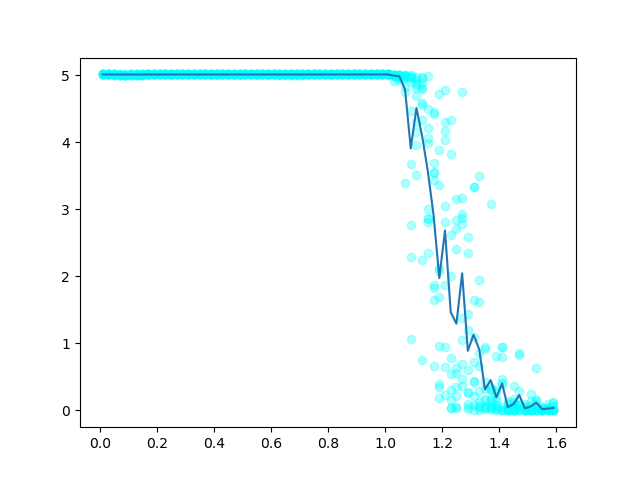
\includegraphics[width=0.6\textwidth]{../L_5.png}
		\caption{$L=5$}
	\end{figure}
	
	Vidíme, že pamäťová kapacita je pomerne stabilne okolo $TMC=5$ pre všetky hodnoty spektrálneho polomeru menšieho ako $1$, pre hodnoty väčšie ako jedna pamäťová kapacita rapídne klesá. 
	\\
	
	Teraz skúsme o niečo vyššiu hodnotu $L=20$, dostaneme takýto graf:
	
	\begin{figure}[!h]
		\centering
		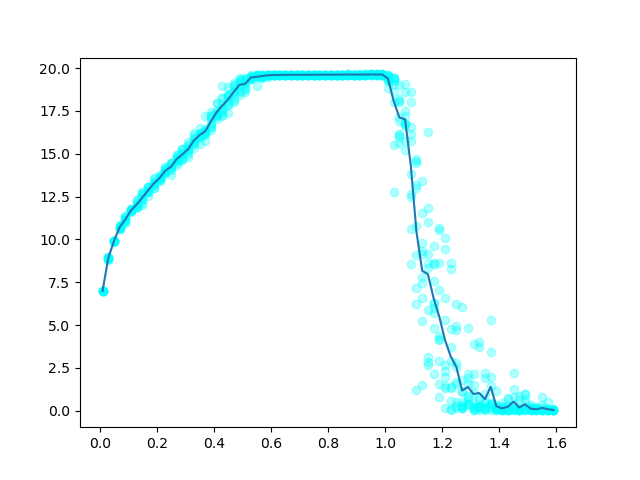
\includegraphics[width=0.6\textwidth]{../L_20.png}
		\caption{$L=20$}
	\end{figure}

	Vidíme, že pre hodnoty spektrálneho polomeru v intervale $\rho \in (0, 0.5)$ pamäťová kapacita postupne rastie, následne pre hodnoty v intervale $\rho \in(0.5, 1)$ je viac-menej na stabilnej maximálnej hodnote približne $TMC=19.6$, a pre hodnoty väčšie ako $1$ začína pamäťová kapacita rapídne klesať a okolo hodnoty $1.5$ je už blízka $0$.
	\newpage
	
	Keďže máme stále pomerne široký interval kedy nastáva maximálna pamäťová kapacita skúsme hodnotu $L$ zvýšiť na $L=40$:
	
	\begin{figure}[!h]
		\centering
		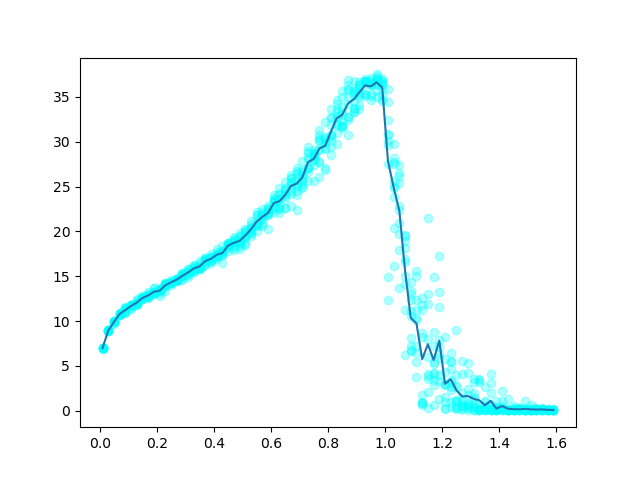
\includegraphics[width=0.6\textwidth]{../L_40.png}
		\caption{$L=40$}
	\end{figure}

	Tu už vidíme, že maximálnu pamäťovú kapacitu $TMC=36.6$ dosiahne pre hodnotu spektrálneho polomeru $\rho=0.97$, inak je správanie podobné prechádzajúcim prípadom kde do tejto hodnoty pamäťová kapacita postupne rastie a od tejto hodnoty prudko klesá.
	\\
	
	Môžeme skúsiť hodnotu ešte zvýšiť a skúsiť $L=80$:
	
	\begin{figure}[!h]
		\centering
		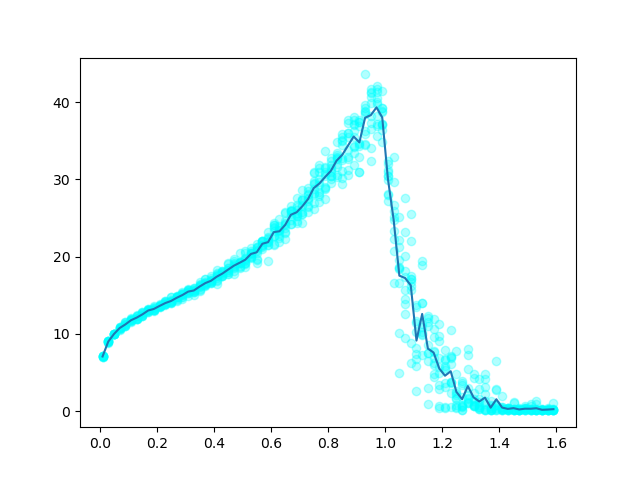
\includegraphics[width=0.6\textwidth]{../L_80.png}
		\caption{$L=80$}
	\end{figure}
	
	Vidíme, že graf je takmer totožný tomu pre $L=40$, maximálna pamäťová kapacita je približne $TMC=39.8$ čo je zaujímavé keďže doteraz bola pamäťová kapacita len o trochu menšia ako hodnota $L$ ale v tomto prípade je len približne polovičná. 
	\newpage
	
	Skúsme sa pozrieť na hodnoty maximálnej pamäťovej kapacity pre $L$ medzi $10$ a $100$ po násobkoch $10$:
	
	\begin{table}[!h]
		\begin{tabular}{|p{0.22\textwidth}|p{0.05\textwidth}|p{0.05\textwidth}|p{0.05\textwidth}|p{0.05\textwidth}|p{0.05\textwidth}|p{0.05\textwidth}|p{0.05\textwidth}|p{0.05\textwidth}|p{0.05\textwidth}|p{0.05\textwidth}|}
			\hline
			L& 10& 20& 30& 40& 50& 60& 70& 80& 90& 100 \\ \hline
			pamäťová kapacita & 9.9& 19.6& 28.9& 36.6& 39.3& 39.4& 39.6& 39.8& 40& 40\\ \hline
		\end{tabular}
	\end{table}
	
	Vidíme, že pamäťová kapacita spočiatku rastie s hodnotou $L$ ale následne sa tento rast spomaľuje až dosiahne úplné maximum okolo hodnoty $TMC=40$. Keďže spočiatku je kapacita podobná hodnote $L$ a jej maximum je $TMC=40$, do ďalšej časti použijeme $L=40$.
	
	\subsection*{Nastavenie $\rho$}
	
	Zopakujme si aký graf sme dostali pre $L=40$:
	
	\begin{figure}[!h]
		\centering
		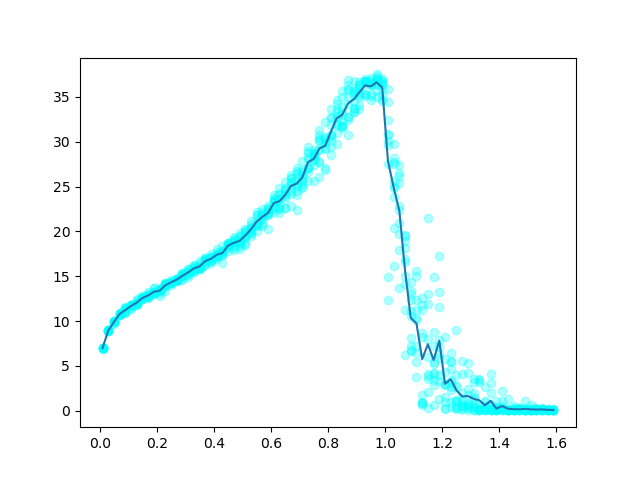
\includegraphics[width=0.6\textwidth]{../L_40.png}
		\caption{$L=40$}
	\end{figure}

	Maximálnu hodnotu pamäťovej kapacity $TMC=36.6$ sme dostali pre hodnotu spektrálneho polomeru $\rho=0.97$, preto ďalej už budeme pracovať s modelom využívajúcim práve túto hodnotu. 
	\\
	
	Teraz sa pozrime na to aká je pamäťová kapacita pre jednotlivé časové oneskorenia, na to aby sme dostali hodnotnejšie výsledky, tento model spustíme 20 krát a vykreslíme boxplot pre jednotlivé oneskorenia, z toho dostaneme takýto graf:
	
	\begin{figure}[!h]
		\centering
		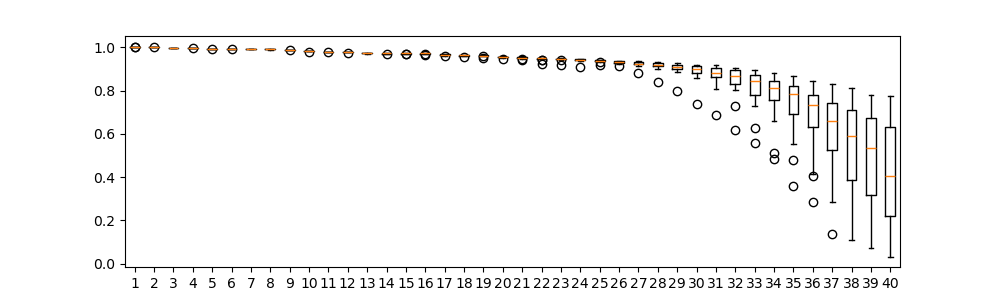
\includegraphics[width=0.9\textwidth]{../box_L_40.png}
		\caption{Boxplot pre $L=40$ a $\rho=0.97$}
	\end{figure}
	
	Môžeme vidieť, že so zväčšujúcim sa oneskorením sa znižuje pamäťová kapacita a zároveň sa zväčšuje rozptyl. Pamäťová kapacita prvých 30 oneskorení je pomerne stabilná s hodnotou $MC_l>0.9$ a následne začína hodnota $MC_l$ výraznejšie klesať a pre oneskorenie 40 je len $MC_{40}\approx 0.4$.
	\\
	
	Tento pokles pamäťovej kapacity pre väčšie oneskorenia by mohol vysvetliť prečo pre $L>50$ vidíme stagnáciu celkovej pamäťovej kapacity, preto si na podobnom grafe zobrazme ako vyzerá pamäťová kapacita pre $L=100$ (najlepší spektrálny polomer bol v tomto prípade podobne ako v predchádzajúcom prípade $\rho=0.97$):
	
	\begin{figure}[!h]
		\centering
		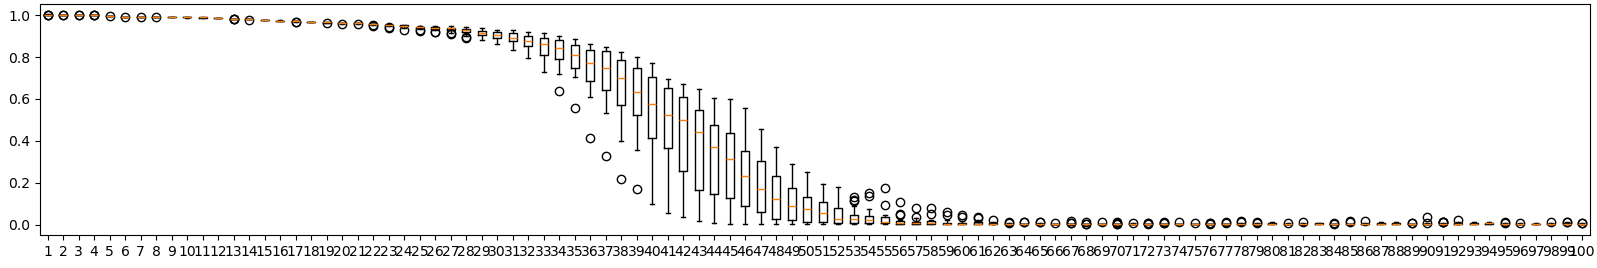
\includegraphics[width=\textwidth]{../box_L_100.png}
		\caption{Boxplot pre $L=100$ a $\rho=0.97$}
	\end{figure}
	
	Z grafu vidíme, že medzi oneskoreniami 30 a 60 klesá v tvare podobnom sigmoide a od oneskorenia 60 je už takmer nulová, čo vysvetľuje zanedbateľný nárast celkovej pamäťovej kapacity pre $L>50$.
	
	\subsection*{Vplyv riedkosti}
	
	Na záver sa pozrieme na to aký vplyv má riedkosť $\tau$, čiže pravdepodobnosť vynulovania hodnoty v matici rezervoáru na pamäťovú kapacitu. Na tento účel použijeme model s parametrom $L=40$ a spektrálnym polomerom $\rho=0.97$. Vizualizujeme si pamäťovú kapacitu pre riedkosť od $0$ (bez vynulovávanie) po $0.99$ (takmer nulová matica) s krokom $0.01$, pričom podobne ako predtým, pre každú hodnotu natrénujeme 10 modelov a vypočítame priemer ich celkových pamäťových kapacít. Z toho dostaneme takýto graf:
	
	\begin{figure}[!h]
		\centering
		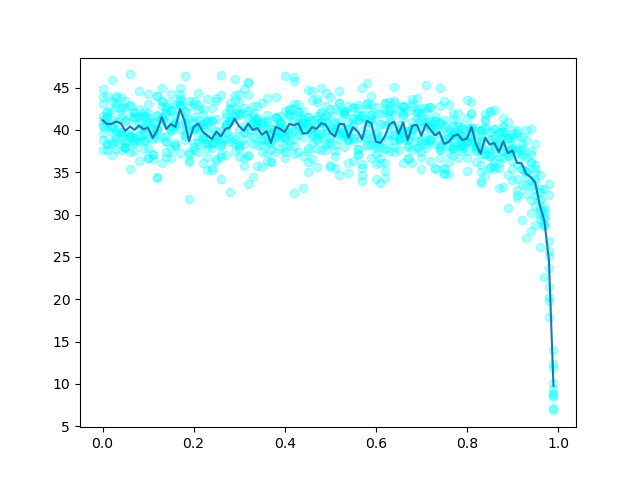
\includegraphics[width=0.6\textwidth]{../spars_L_100.png}
		\caption{$L=40$ a $\rho=0.97$}
	\end{figure}
	
	Vidíme, že riedkosť v intervale $\tau \in (0, 0.8)$ nemá veľký vplyv na pamäťovú kapacitu modelu, nanajvýš sa môže zdať, že zo zvyšujúcou sa riedkosťou sa mierne kapacita zmenšuje ale je to nevýrazné. Avšak pre riedkosť $\tau > 0.8$ vidíme, že nastáva výrazný pokles pamäťovej kapacity a pre $\tau = 0.99$ sa už blíži k nule. Toto dáva zmysel, keďže vysoké hodnoty riedkosti znamená že matica rezervoáru ná iba malý počet nenulových hodnôt čiže neuróny sú veľmi málo prepojené. 
	
\end{document}